\documentclass{amsart}

\synctex=1

\usepackage{amsmath,amsthm,amssymb}
\usepackage{todonotes}
\usepackage[notref,notcite]{showkeys}
\usepackage{enumerate}
\usepackage{url}
\usepackage[hidelinks]{hyperref}
\usepackage{graphicx}
\usepackage[style=authoryear-icomp,ibidtracker=false]{biblatex}

\addbibresource{curvatureNNI.bib}

\newtheorem{lemma}{Lemma}
\newtheorem{question}[lemma]{Question}
\newtheorem{proposition}[lemma]{Proposition}
\newtheorem{corollary}[lemma]{Corollary}
\newtheorem{theorem}[lemma]{Theorem}
\newtheorem{problem}[lemma]{Problem}

\theoremstyle{definition}
\newtheorem{example}[lemma]{Example}
\newtheorem{conjecture}[lemma]{Conjecture}

\newcommand{\dts}{\mathrm{2DtT}}
\newcommand{\nni}{\mathrm{NNI}}
\newcommand{\rnni}{\mathrm{rNNI}}
\newcommand{\rnniu}{\mathrm{rNNIu}}
\newcommand{\mdts}{\mathrm{DtT}}
\newcommand{\mdtsu}{\mathrm{DtTu}}
\newcommand{\MH}{\mathrm{MH}}
\newcommand{\ric}{\operatorname{ric}}
\newcommand{\rt}{\operatorname{rt}}
\newcommand{\tp}{\operatorname{tp}}
\newcommand{\W}{\mathcal{W}}
\newcommand{\M}{\mathcal{M}}
\newcommand{\dom}{\operatorname{dom}}
\newcommand{\G}{\mathcal{G}}

\renewcommand{\O}{\mathcal{O}}

\sloppy

\begin{document}

\title{Random walks over discrete time-trees}

\author{Alex Gavryushkin}
\address{Department of Computer Science, The University of Auckland, New Zealand}
\email{a.gavruskin@auckland.ac.nz}

\author{Chris Whidden}
\address{Program in Computational Biology, Fred Hutchinson Cancer Research Center, Seattle, WA 98109}
\email{cwhidden@fredhutch.org}

\author{Frederick A Matsen IV}
%\address{Program in Computational Biology, Fred Hutchinson Cancer Research Center, Seattle, WA 98109}
\email{matsen@fredhutch.org}


\begin{abstract}
We introduce and study various discrete approximations of the space of time-trees, with $\nni$-space being a roughest approximation.
We design a heuristic for generating these spaces and study, analytically and computationally, the Ricci-Ollivier curvature of basic random walks on the spaces.
\end{abstract}


\maketitle


\section{Introduction}
The last ten years have seen an explosion of methods using sequence data to infer demographic model parameters by sampling phylogenetic trees \autocite{Kuhner1995-mj,Kuhner1998-tq,Kuhner2000-af,Beerli2001-sc,Kuhner2006-vx,Drummond2002,Drummond2005-ks,Drummond2006-oa,Minin2008-wz}.
Dates defined in phylogenetic terms, such as time to a most recent common ancestor of human HIV group M viruses \autocite{Worobey2008-rt,Baele2013-op}, are essential parameters of such inference.
Thus the {\em time-tree}---a rooted phylogenetic tree with all internal nodes equipped with absolute divergence dates---has become an important object of interest.
This is in contrast to classical phylogenetic trees in which branch lengths quantify the amount of molecular substitution along a branch.
Posterior distributions on both time-trees and classical trees are estimated using Markov chain Monte Carlo \autocite{Mau1997-sq,Yang1997-gv,Drummond2002}.
Although Markov chain Monte Carlo (MCMC) is guaranteed to sample from the true posterior given an infinite run time, it is important to understand mixing properties of the chain, which determine sampling properties for a finite time run.

\begin{figure}[ht]
\centering
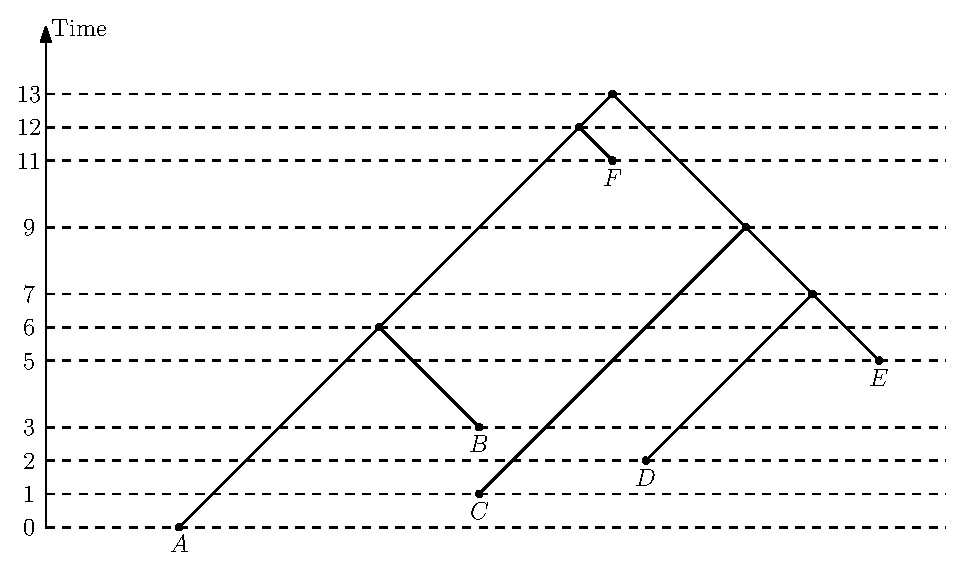
\includegraphics[width=0.7\textwidth]{timeTree.eps}
\caption{Time tree on $6$ taxa.
Time is measured by nonnegative real numbers.}
\label{timeTree.eps}
\end{figure}

The mixing properties of phylogenetic MCMC have, in the classical unrooted case, been a major area of research from both the theoretical perspective of mixing time bounds \autocite{Mossel2005-ly,Mossel2006-fo,Stefankovic2011-hu,spade2014note} and the practical perspective of performance on real data \autocite{beiko2006searching,Ronquist2006-fv,lakner2008efficiency,Whidden2015-yi}.
This research has focused on mixing over the set of discrete phylogenetic tree graph structures, which is the primary obstruction to MCMC convergence.
Classical phylogenetic trees discretize naturally as simply the graph structure underlying that phylogenetic tree.
MCMC moves between classical phylogenetic trees are typically defined in terms of this discretization.
Common moves include \emph{subtree prune and regraft} (SPR) moves, which cut a subtree off and reattach it at another location, and the subset of SPR moves called \emph{nearest-neighbor interchange} (NNI) moves.
On the other hand, moves between time-trees are also defined in terms of their timing information.
For example, \textcite{Hohna2008-vl} show that SPR-like moves that reattach subtrees at the same divergence time are more effective than ones that do not.
This sort of move cannot be expressed using the type of discretization used thus far in which all continuous information is lost, and so the previous work on MCMC mixing cannot be applied.

However, one can discretize time-trees in a way that does preserve some of the information.
For example, by retaining the order of internal nodes backward in time one obtains a so-called \emph{ranked tree} \autocite{Semple2003-nj}.
A sequence of time-trees sampled using MCMC projects to a collection of movements on a graph in which each vertex is a discretized time-tree and each edge is a discretized version of an MCMC move on time-trees.

Another possible way to make a less rough approximation of a time-tree is to allow the time periods between nodes of the tree to take only finitely many possible values.
The graph built on such trees provides a further refined discretization of the space of time-trees.
We call such a graph a \emph{discretized time-tree graph}.

In this paper we explore various discretized time-tree graphs, derive some of their properties, initiate the mathematical study of random walks on these spaces, and compare these results to those in the classical phylogenetic setting.
In particular, we focus on ranked trees, discretized time-trees (as defined above), and the ultrametric versions of those types of trees.
We study Ricci-Ollivier curvature \autocite{Ollivier2009-cj} of Markov chains on these graphs, a formalism which quantifies to what extent random walking brings unit balls together.
This formalism has recently been applied to Markov chains on graphs of classical phylogenetic trees \autocite{Whidden2015-es}.


\section{Technical introduction}
\subsection{Spaces of discretized time-trees}

By a {\em time-tree} we mean a rooted phylogenetic tree with all internal nodes equipped with absolute divergence times and all external nodes equipped with sampled times.
As a first step toward understanding the full space of time-trees \autocite{Gavryushkin2014-bw}, we approximate the space by a sequence of finite spaces and study the geometry and convergence of random walks over those approximations.
Specifically, we fix a number $m$ and consider the space of time-trees where times between divergence events are bound to $m$ values.
At the bottom level of this hierarchy, when $m = 1$, we have the space of ranked tree topologies.
We extend the hierarchy by assuming that when $m = 0$, we have the $\nni$ space on rooted tree topologies.

Many biological investigations are restricted to ultrametric, or equidistant, trees: trees for which the distance of every leaf to the root is the same.
Furthermore, many geometric and algorithmic properties differ substantially between ultrametric and non-ultrametric trees, as shown by \textcite{Gavryushkin2014-bw}.
Hence, we consider the case of ultrametric trees separately, and indeed establish further differences.

In short, the {\em discrete time-tree space,} or $\mdts$ space, is the
$\tau$-space\footnote{Note that (interestingly) discretized versions of $\tau$- and $\mathrm t$-space from \autocite{Gavryushkin2014-bw} coincide.}
defined by \textcite{Gavryushkin2014-bw}, where the real-valued parameters (length intercoalescent intervals) are allowed to take only $m$ possible values: $1,\ldots,m$.
In other words, to define a tree in $\mdts$, we first fix a ranked tree topology with all nodes being of different ranks and then assign a number from $\{1, \ldots, m\}$ to every intercoalescent interval.
Intuitively, for $m = 2$ we have only two options for the length of an intercoalescent interval, which can be thought of as short and long.
We shall describe the integers assigned to the intercoalescent intervals as {\em lengths} of those intervals.

We may think of the $\mdts$ space as of a graph, the set of vertices of which consists of $\mdts$ trees, and define the adjacency relation as follows.
In short, two trees in $\mdts$ are adjacent if the $\tau$-geodesic between them, as defined by \textcite{Gavryushkin2014-bw}, crosses precisely one face and the face is of co-dimension $1$.
To make this paper self-contained, we provide a complete definition below.

Let $T$ be a time-tree such that no two nodes of $T$ are of the same time, that is, no two divergence or sample events coincide.
We define the {\em ranked topology of tree} $T$ to be the (directed) graph induced by the topology of $T$ such that the set of nodes of this graph is linearly ordered with respect to their time order in $T$.
We denote this ranked topology by $\rt(T)$ and assume that all nodes of the tree (including taxa) are assigned ranks $0,1,\ldots,2n-2$, where $n$ is the number of taxa.
The node of rank $0$ is seen as being at the present, so the root has the highest rank and is therefore the oldest node of the tree.
An {\em intercoalescent interval} of $T$ is an interval between any two nodes of consecutive ranks (Figure~\ref{T5.pdf}).
By $\ell_T(I)$ we denote the length of intercoalescent interval $I$ in tree $T$.
We say that two trees $T$ and $R$ {\em have the same ranked topology} and write $\rt(T) = \rt(R)$ if the tree topologies are isomorphic as (directed) graphs and the isomorphism preserves ranks of the nodes.
In the same way we write $\tp(T) = \tp(R)$ when trees $T$ and $R$ have the same rooted tree topology (that is, ranks are ignored).

\begin{figure}[ht]
\centering
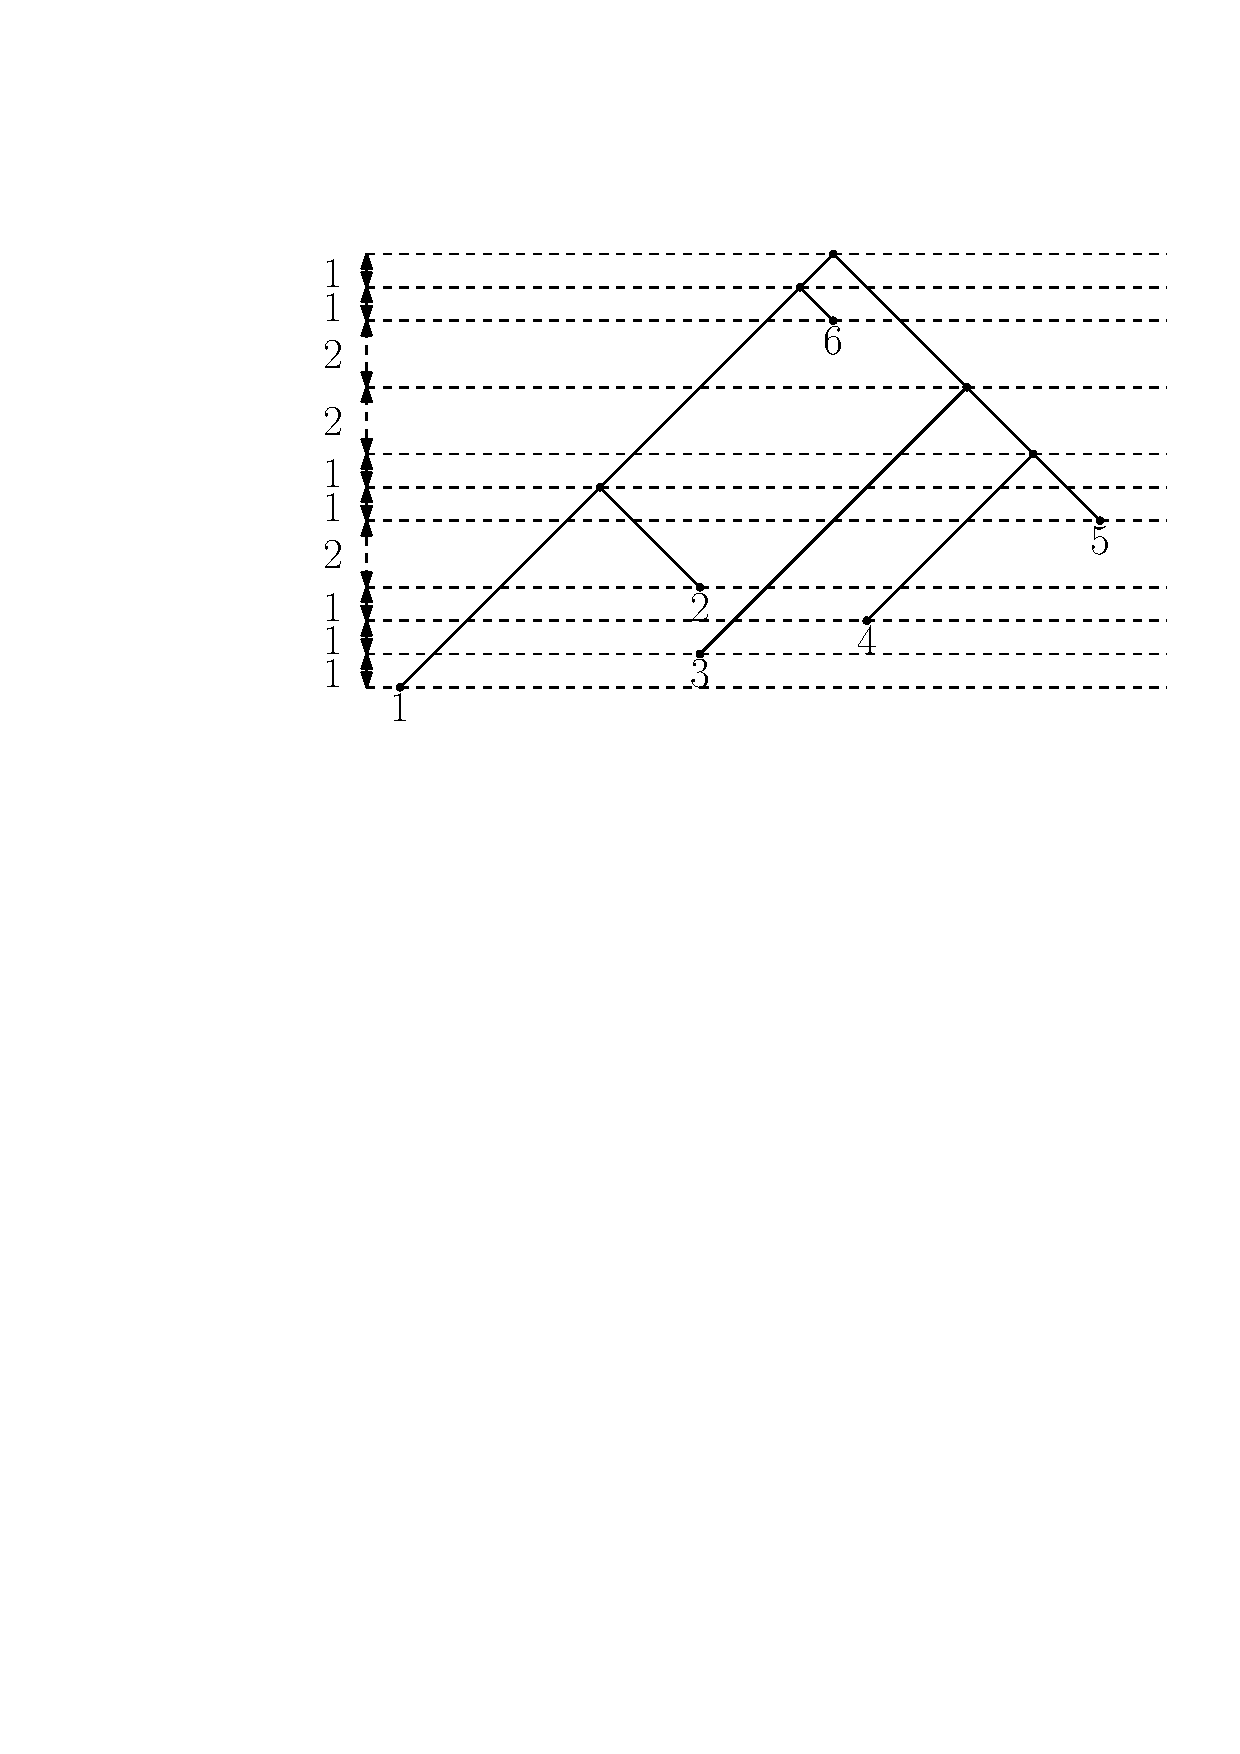
\includegraphics[width=0.7\textwidth]{T5.pdf}
\caption{Discretized time-tree on $6$ taxa.
Intervals between divergence and sample events can take only finitely many values (two in this example).}
\label{T5.pdf}
\end{figure}

We say that two trees $T$ and $R$ are {\em NNI neighbors} if $\rt(T) \ne \rt(R)$ and tree $R$ is obtained from tree $T$ by sending the length of an intercoalescent interval $I$ between an internal node and its parent in $T$ down to zero and resolving the multifurcation in one of the two possible ways.
We note that this definition implies the existence of such an interval $I$ in $T$, that is, the existence of an internal node $a$ the parent of which is the immediate successor of $a$ in $\rt(T)$.
In particular, the parent $a$ of taxon $D$ in tree $T$ on Figure~\ref{dts_neighbors.pdf} gives an example of such a node.
Note also that the parent $b$ of taxon $C$ in $T$ on Figure~\ref{dts_neighbors.pdf} does not satisfy this property, that is, the parent of $b$ is not its immediate successor in $\rt(T)$.
Hence, the tree obtained from $T$ by cutting the edge adjacent to taxon $C$ and regrafting it to the edge between the aunt of $b$ and the root does not give an NNI neighbor of $T$ in this sense.
Note that the definition of NNI neighbors implies $\ell_T(J) = \ell_R(J)$ for each interval $J \ne I$, and the ranks of all nodes present in both $T$ and $R$ coincide.
If trees $T$ and $R$ are NNI neighbors and tree $R$ is obtained by suppressing an interval $I$ in $T$ then we say that the {\em NNI move is performed on interval $I$}.

Two trees $T$ and $R$ from $\mdts$ are adjacent if and only if precisely one of the following conditions is satisfied.
\begin{enumerate}[(1)]
\item $\rt(T) = \rt(R)$ and there exists a unique intercoalescent interval $I$ such that $|\ell_T(I) - \ell_R(I)| = 1$.
\item $\tp(T) = \tp(R)$, there exists a unique pair of nodes $a,b$ with consecutive ranks in $\rt(T)$ such that the ranks of $a$ and $b$ are swapped in $R$, the intercoalescent interval $I$ between $a$ and $b$ satisfies $\ell_T(I) = \ell_R(I) = 1$, and $\ell_T(J) = \ell_R(J)$ for all other intervals $J \ne I$.
\item $T$ and $R$ are NNI neighbors and $\ell_T(I) = \ell_R(I) = 1$ where the NNI move is performed on interval $I$.
\end{enumerate}

In other words, by going from one tree to an adjacent tree in the $\mdts$ graph we can either change the length of one intercoalescent interval by one unit, swap the rank of two nodes, or send the length of an intercoalescent interval of minimal length down to zero and then resolve the multifurcation to either of the two possible topologies.
In the latter case, the new interval is of minimal length.
See Figure~\ref{dts_neighbors.pdf} for an example of a pair of trees $T,R$ at $\mdts$ distance $3$, where one has to apply all of the three possible cases from the definition above to obtain a path from $T$ to $R$ in $\mdts$.

\begin{figure}[ht]
\centering
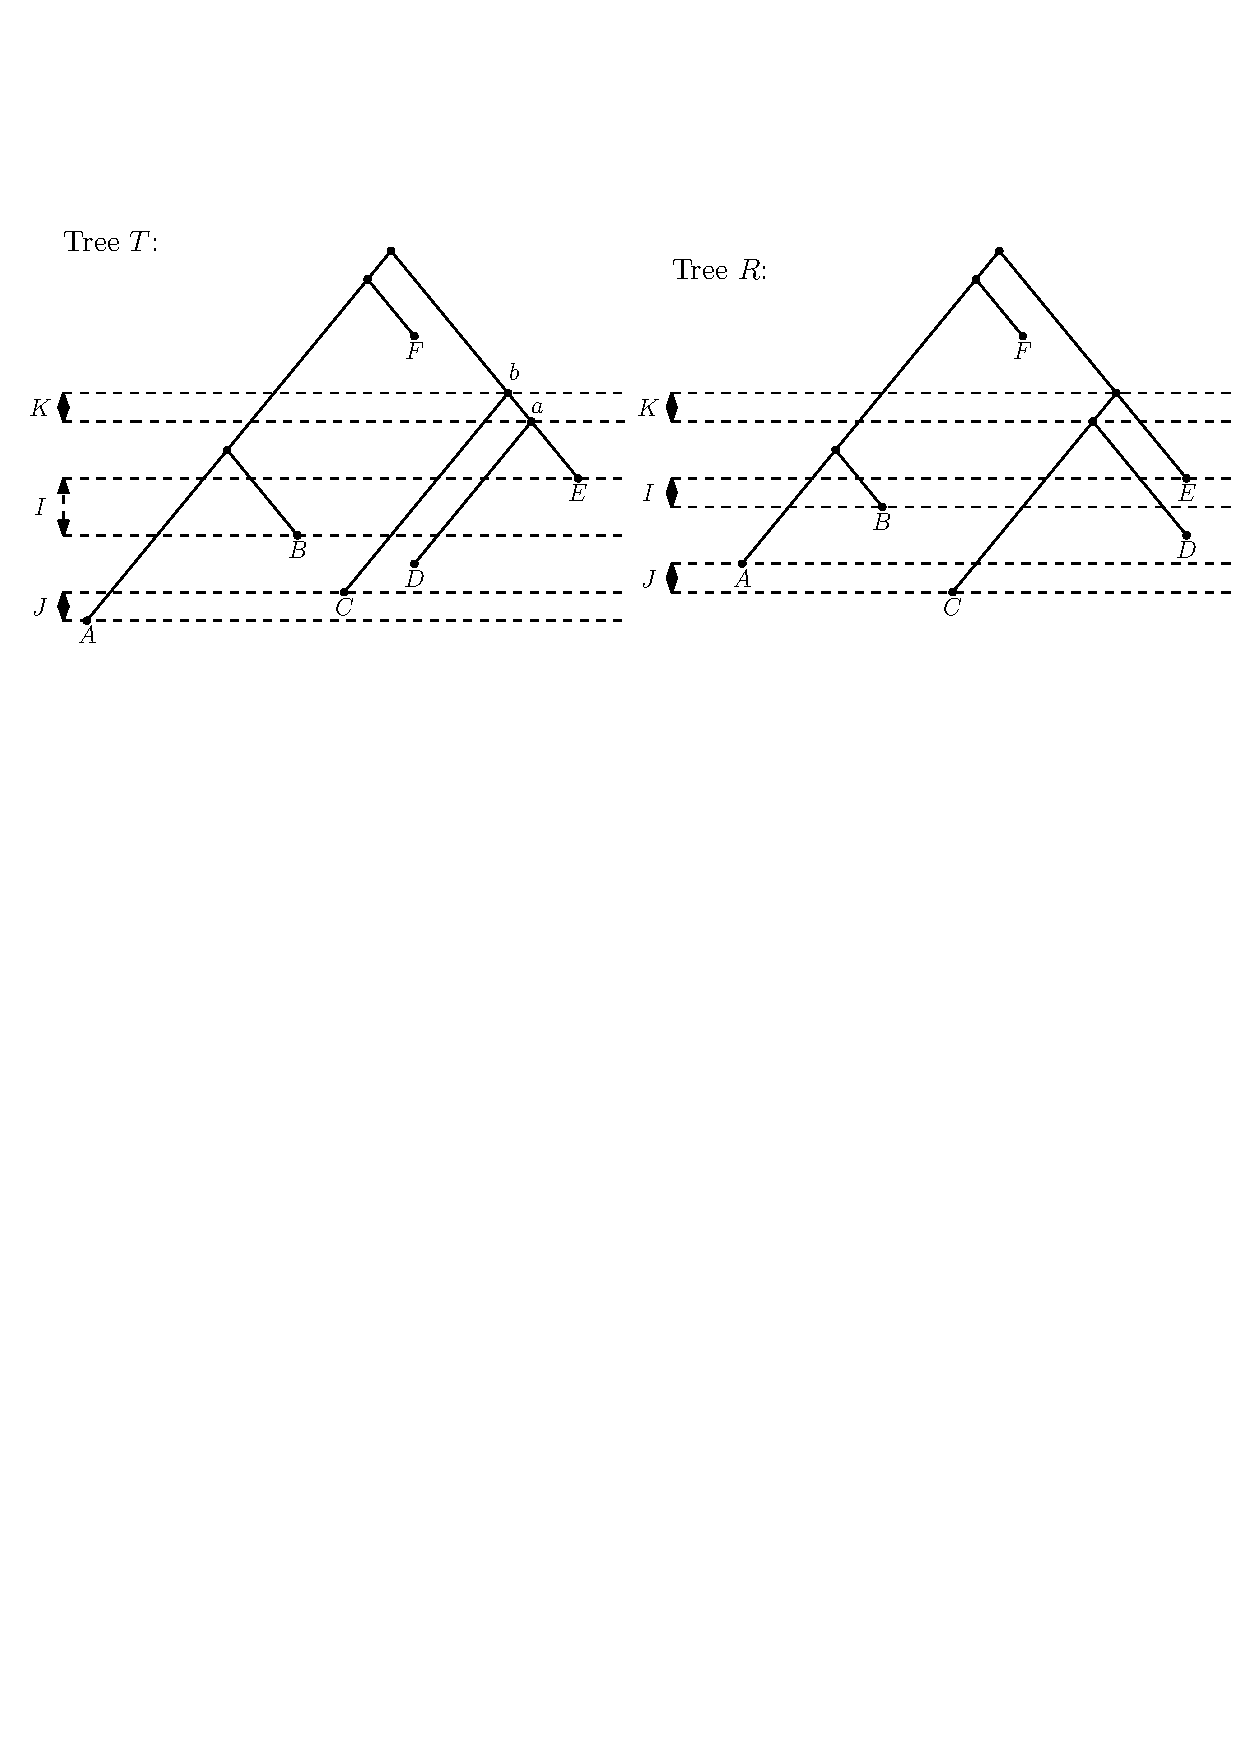
\includegraphics[width=0.7\textwidth]{dts_neighbors.pdf}
\caption{Trees $T$ and $R$ are at $\mdts$ distance $3$.
To move from $T$ to $R$ in $\mdts$, one must decrease the length of interval $I$, swap the ranks of nodes $A$ and $C$ bounding the interval $J$, and perform an NNI move on interval $K$, resolving nodes $C$ and $D$.}
\label{dts_neighbors.pdf}
\end{figure}

Thus we have defined a graph, which we denote by $\mdts$ for $m \geq 2$.
Since a graph can also be seen as a metric space where the distance is given by the length of a shortest path, we will refer to $\mdts$ as both.

One might suggest that geometrically and graph-theoretically $\mdts$ is similar to NNI space on (rooted) tree topologies, to ranked NNI space, and to $\mdts$ space on ultrametric trees.
That is so indeed.
As we shall see, the results and proofs in this paper can be straightforwardly adapted to the spaces mentioned.
Furthermore, as the NNI space of unrooted tree topologies with $n-1$ leaves is isomorphic (as a graph) to the NNI space of rooted tree topologies with $n$ leaves, all our results immediately imply their counterparts in unrooted NNI space.
We omit from the text the exact formulations for unrooted trees, as they can be obtained in the obvious way.
We will provide complete proofs for $\mdts$ space and draw the corresponding results for the other three treespaces simultaneously.

The $\mdts$ space on ultrametric trees is denoted by $\mdtsu$.
The $\mdts$ space (on ultrametric trees) with only short branches is denoted by $\rnni$ ($\rnniu$) and called {\em ranked NNI} space (on ultrametric trees).
The $\nni$ space on rooted tree topologies is denoted by $\nni$.

All of these can be considered as either a graph or a metric space, and we will refer to them as both.
By $n$ we denote the number of taxa and assume $n \geq 3$ throughout the paper.


\subsection{Ricci-Ollivier curvature}
A random walk on a metric space is defined by its proposal mechanism, which is a functional $m$ that maps points of the space to the set of measures on this space \autocite[see][]{Ollivier2009-cj}.
In other words, for every point $v$ in the space, $m(v,w)$, which we denote by $m_v(w)$, is the probability of the random walk moving from $v$ to $w$ in one step.
Given a metric space $(V,d)$, a \emph{coupling} $\mu$ between two measures $\mu_1$ and $\mu_2$ on $V$ is a probability measure on the set of pairs of points $V \times V$ that is $\mu_1$ after marginalizing over the second component, and $\mu_2$ after marginalizing over the first component, that is, $\sum\limits_{y \in V}\mu(x,y) = \mu_1(x)$ and $\sum\limits_{y \in V}\mu(y,x) = \mu_2(x)$ for all $x \in V$.
A coupling can be seen as a scenario of transforming the measure $\mu_1$ on $V$ to $\mu_2$ by looking at $\mu(x,y)$ as the probability mass that has to be moved from $x$ to $y$ under the scenario.

Using these notations, we define the {\em work} $\W_\mu$ needed to be done to transform $\mu_1$ to $\mu_2$ via coupling $\mu$ by setting
\[
\W_\mu(\mu_1,\mu_2) = \sum\limits_{x,y\in V}\mu(x,y) d(x,y).
\]
Let $\M$ be the set of all couplings between measures $\mu_1$ and $\mu_2$.
Then the {\em earth mover's distance} $W$ between $\mu_1$ and $\mu_2$ is defined to be $W(\mu_1,\mu_2) = \inf\limits_{\mu\in\M}\W_\mu(\mu_1,\mu_2)$.

We are now ready to introduce two curvature notions that we are studying in this paper.
Let $m$ be a random walk on a metric space $(V,d)$.
Then the {\em coarse Ricci-Ollivier curvature} between two points $x$ and $y$ from $V$ with the random walk $m$ is
\[
\kappa(m;x,y) = 1 - \frac{W(m_x,m_y)}{d(x,y)}
\]

Another important notion of this paper is that of asymptotic curvature.
The following random walk $m$ is called a {\em uniform $p$-lazy random walk} on a metric space $(V,d)$:
\[
m_x(y) =
\begin{cases}
1-p			& \mbox{ if } x=y \\
0   			& \mbox{ if } d(x,y) > 1 \\
\dfrac{p}{|N(x)|}	& \mbox{ if } d(x,y) = 1 \\
\end{cases}
\]
where $x,y \in V$ and $N(x) = \{y \mid d(x,y) = 1\}$.

We follow \textcite{Loisel2014-gu} and define {\em asymptotic Ricci-Ollivier curvature} $\ric$ between points $x,y$ from a metric space with uniform $p$-lazy random walk $m$ by
\[
\ric(x,y) = \lim_{p\to0} \frac{\kappa(m;x,y)}{p}
\]

One of the central properties of Ricci-Ollivier curvature is that the curvature is a local property \autocite{Ollivier2009-cj}.
For finite metric spaces that means that for all distinct $u$ and $v$,
\[
\inf\{\kappa(m;x,y)\mid d(x,y) = 1\} \leq \kappa(m;u,v).
\]
Hence, we define the {\em coarse Ricci-Ollivier curvature of a metric space} with a random walk $m$ to be $\inf\{\kappa(m;x,y)\mid d(x,y) = 1\}$ and the {\em asymptotic Ricci-Ollivier curvature of a metric space} to be $\inf\{\ric(x,y)\mid d(x,y) = 1\}$.


\section{Geometry of space of discrete time-trees}

We begin with considering the shortest path distance on the graphs.
It is well-known that computing distance is NP-hard in $\nni$ space \autocite{Dasgupta2000-xa}.
Hence, for each of the possible discretizations of the time-tree space, a natural question is the following.

\begin{problem}
What is the complexity of computing the distance between two discrete time-trees?
\end{problem}

Although we do not solve this problem in this paper, we demonstrate that the solution could be different for different versions of time-trees.
Particularly, we demonstrate in the following example that even for caterpillar trees the solution could be non-obvious.

\begin{example}
Let $T$ be the ultrametric tree $((((((1, 2), 3), 4), 5), 6), 7)$ and $R$ be the ultrametric tree $((((((1, 4), 5), 6), 2), 3), 7)$.
Then a shortest $\nni$ path is given by first making a cherry $(2,3)$, then moving the cherry up to the split $1456 \mid 7$, and then resolving the cherry back.
While in $\rnniu$ this path is not shortest, and a shortest path would be to move up the parents of $2$ and $3$ independently.

\begin{figure}[ht]
\centering
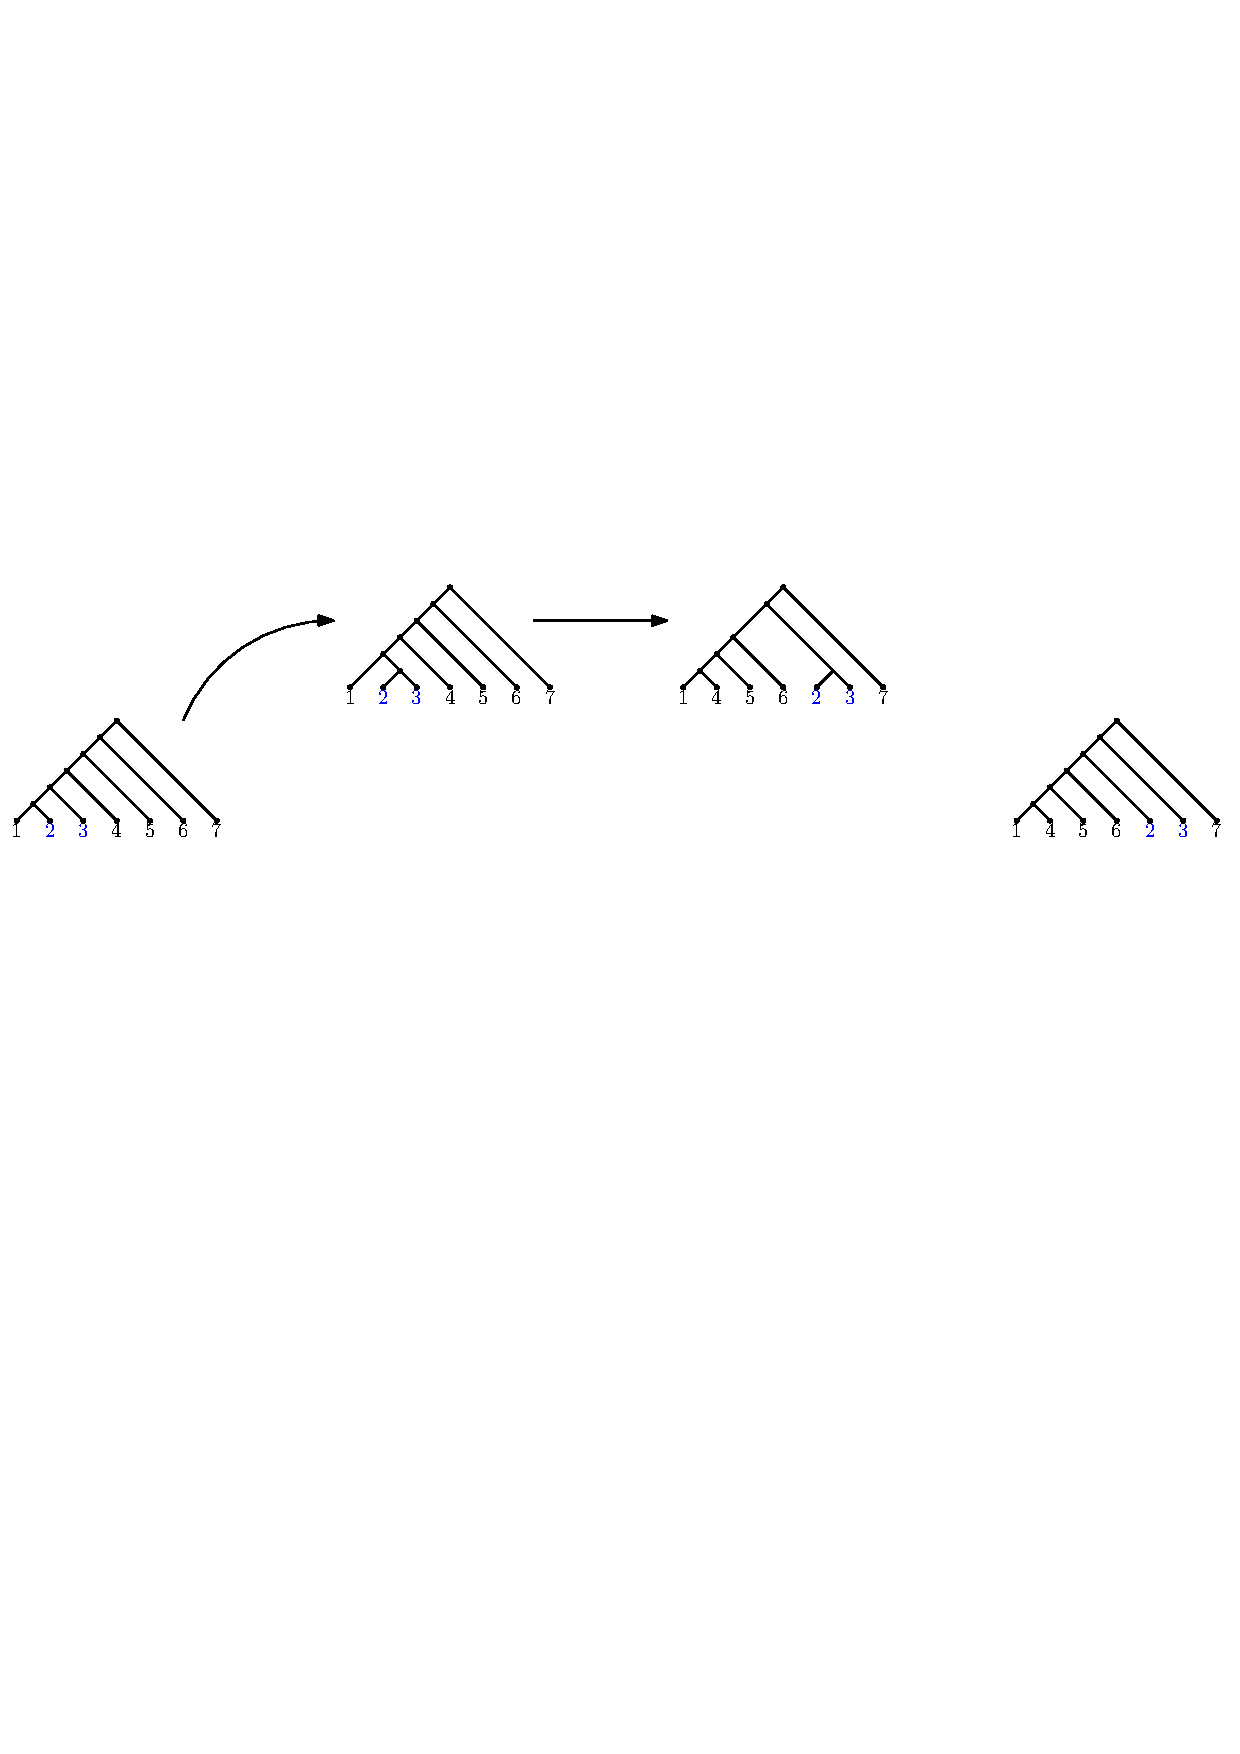
\includegraphics[width=\textwidth]{NNI_VS_rNNI.pdf}
\caption{No shortest $\nni$ path is shortest in $\rnni$.}
\label{NNI_VS_rNNI.pdf}
\end{figure}
\end{example}

With this example in mind, it is not hard to see that the set of trees of the form $(\ldots(1, i_2), \ldots, i_{n-1}), n)$, where $\{i_2, \ldots, i_{n-1}\} = \{2, \ldots, n-1\}$, is convex in the space of discrete time-trees and is not convex in $\nni$.

The following theorem bounds the sizes of neighborhoods.

\begin{theorem}\label{neighSizeTh}
The number of trees within distance $r$ from any given tree is at most
\begin{itemize}
\item[] $3^{n+2r-1}$ in $\rnniu$,
\item[] $3^{2n+2r-2}$ in $\rnni$,
\item[] TBA in $\mdts$,
\item[] TBA in $\mdtsu$.
\end{itemize}
\end{theorem}

\proof
We prove the theorem in $\rnniu$ and it will follow similarly in the other three spaces.

The proof employs the technique from \autocite{Sleator1992-bp} for counting paths in a graph: we first apply Theorem~2.3 of \textcite{Sleator1992-bp} and then improve the bound using specific properties of $\rnniu$ graph.

We first need to introduce the {\em graph grammar} for $\rnniu$.
Recall that a graph grammar consists of a finite set of productions $\{L_i \to_i R_i\}$, where $L_i$ and $R_i$ are connected undirected edge-end labeled graphs and $\to_i$ is a one-to-one map between half-edges of $L_i$ and those of $R_i$.
See \autocite{Sleator1992-bp} for precise definition.
The graph grammar for $\rnniu$ is then the grammar $\Gamma$ shown on Figure~\ref{grammar_rNNIu.pdf}.
Note that the definition of a graph grammar requires the left sides $L_i$ to be connected and we have a disconnected left side in the third production.
This does not cause a problem because the nodes on the left side of the production must be of consecutive ranks.
(One could think of those nodes as being adjacent via a second type adjacency relation on top of the first type adjacency relation given by the branches of the tree.)

\begin{figure}
\centering
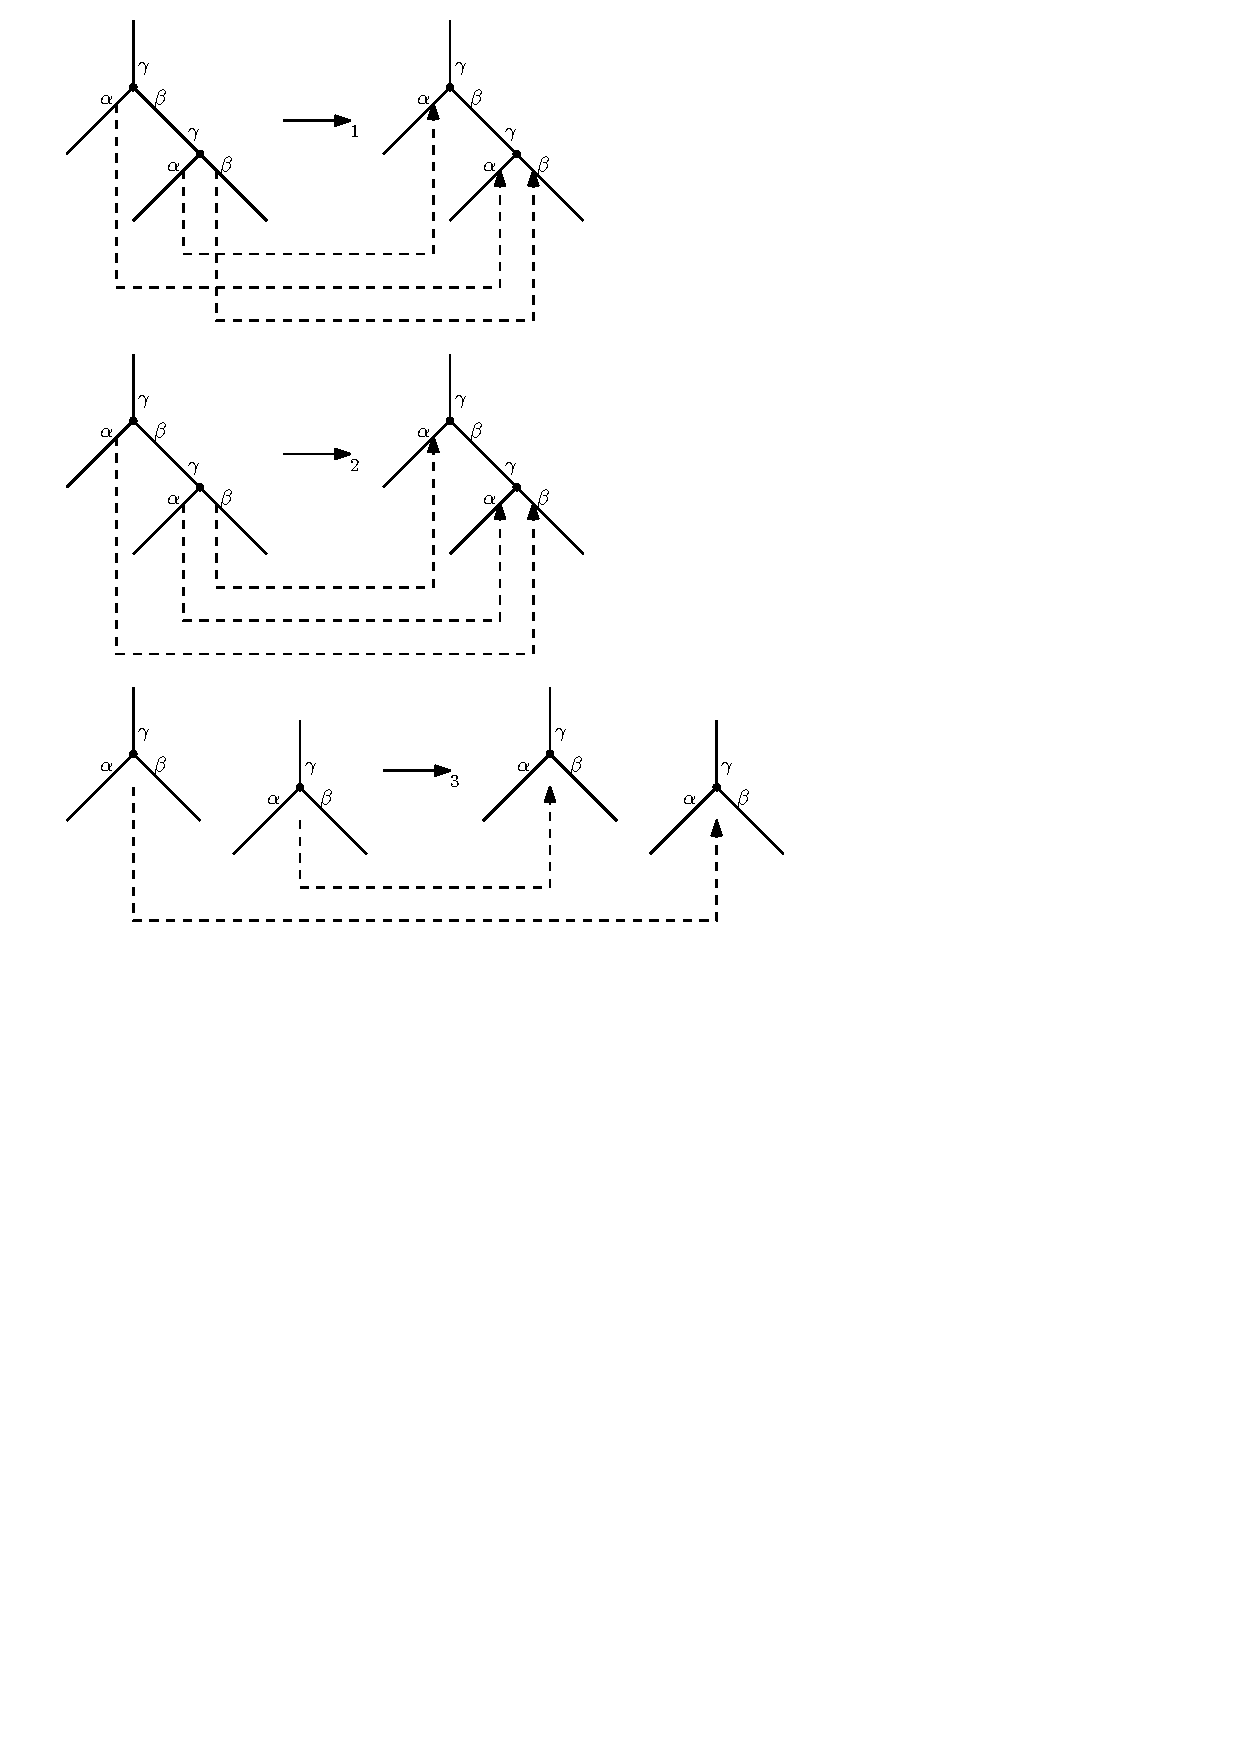
\includegraphics[width=0.7\textwidth]{grammar_rNNIu.pdf}
\caption{Graph grammar $\Gamma$ for $\rnniu$.
Maps $\to_i$ are shown by dashed lines.
Edge-ends labeled by $3$ are mapped top to top, bottom to bottom.
In the last production edge-ends marked by the same label are mapped to each other.
All pairs on nodes on both sides of each production must be on consecutive ranks.
First two productions correspond to $\nni$ move, last production corresponds to rank change.}
\label{grammar_rNNIu.pdf}
\end{figure}

Hence the number of vertices in left sides of $\Gamma$ is $6$, the maximum number of vertices in any right side of a production of $\Gamma$ is $2$.
Since the number of internal nodes of a tree on $n$ leaves in $\rnniu$ is $n-1$, directly applying Theorem~2.3 from \autocite{Sleator1992-bp} we get the bound of $7^{n+2r-1}$.

This bound can be improved following the techniques developed in \autocite{Sleator1992-bp}.
Every node of a tree in any application of a production of grammar $\Gamma$ can play either of two roles: top node or bottom node.
Hence to indicate that a pair of nodes is ready for being replaces using a production, we must specify which node is the top and which is the bottom.
Furthermore, to distinguish which of the two possible $\nni$ moves has to be applied, we must employ another vertex label.
We claim that tree labels $1,2,3$ for the vertices is enough.
Indeed: We say that a pair of consecutive nodes is {\em ready} if the label of the bottom node is $1$ and the label of the top node is either $2$ or $3$.
If two consecutive nodes are ready and not connected by an edge in the tree, then only the rank move is possible.
If they are, the type of the rank move is determined by the label of the top node.

In total, $n-1$ internal nodes result in $3^{n-1}$ possible labelings of the initial tree, plus every application of a production creates two new nodes, each of which can have three possible labelings, hence the improved bound is $3^{n-1} \cdot 3^{2r}$.
\endproof

\begin{conjecture}
\begin{enumerate}[(1)]
The list of conjectures that would nice to settle in this paper:
\item Let $r \le \Delta(\nni)$, then $|\delta_\nni(r, T)| \ge |\delta_\rnni(r, T)|$ for all ranked trees $T$, where $|\delta_\G(d, X)|$ is the number of trees at distance $d$ from $X$ in $\G$.
\item Proposition~\ref{splitPropo}.
\item Lemma~\ref{diameterUpperBound}.
\item Proposition~\ref{isoperiPropo}.
\end{enumerate}
\end{conjecture}

\begin{proposition}\label{splitPropo}
Every split present in both trees $T$ and $R$ presents in all trees along every shortest path between $T$ and $R$ in $\mdts$, $\mdtsu$, $\rnni$, and $\rnniu$, but not in $\nni$.
\end{proposition}

\proof
The counter-example for $\nni$ space is constructed by \textcite{li1996some}.
Hence, we prove the rest.

Suppose there exists a pair of trees $T,R$ sharing a split $A \mid B$ such that no tree on a shortest path between $T$ and $R$ has split $A \mid B$.
Let $T_A$ be the subtree of $T$ on taxa $A$ and $T_B$, $R_A$, $R_B$ are defined analogously.

Road map:
\begin{enumerate}[(1)]
\item We can assume that the size of $A$ is $\lfloor\frac n2\rfloor$.
\item We can assume that there exists trees $\operatorname{join}(T_A, T_B)$ and $\operatorname{join}(R_A, R_B)$ on the shortest path from $T$ to $R$ such that
\[
d(T,\operatorname{join}(T_A, T_B)), d(R,\operatorname{join}(R_A, R_B)) \ge  n^2/8 + n/4.
\]
\item The splitless distance is then at least
\[
n^2/8 + n/4 + d(T_A, R_A) + n^2/8 + n/4
\]
and the length of the path that maintains the split is $2d(T_A, R_A)$.
\item Since the diameter of the space is bounded from above by $15/16n^2$---see Lemma~\ref{diameterUpperBound}---the proposition is proved.
\end{enumerate}
\endproof

A non-ranked tree has a symmetry associated with every internal node.
Those symmetries can be employed to substantially reduce the search space of pairs of trees.
This approach uses tanglegrams \autocite{Matsen2015-fn} and is applied to reduce the number of pairs of tree for computing the curvature \autocite{Whidden2015-es}.
As the following proposition shows, ranked trees are free from all but one of those symmetries, hence the tanglegram approach is not applicable in this case.

\begin{proposition}
Let $T$ be a tree from $\mdts$, $\mdtsu$, $\rnni$, or $\rnniu$ and $\sigma$ a permutation of taxa of $T$.
Let $T_\sigma$ be the tree obtained from $T$ by permuting the taxa using $\sigma$.
Then $T = T_\sigma$ if and only if $\sigma$ is either the identity permutation or a transposition of a pair of taxa that form a
cherry\footnote{A {\em cherry} is a pair of taxa adjacent to a common internal node in the tree.}
in $T$.
\end{proposition}

\proof
The sufficiency is obvious.
For the necessity, assume that $\sigma$ transpose taxa $i,j$ such that $i,j$ is not a cherry in $T$.
This implies that $i$ and $j$ have different parents.
Hence $T \ne T_\sigma$ because the ranks of the parent of $i$ are different in $T$ and $T_\sigma$.
\endproof

These observations suggest that $\nni$ space is geometrically and algorithmically different from the other four spaces.

\begin{lemma}[\textcite{Semple2003-nj}]\label{spaceSizes}
Let $|V|$ be the number of vertices in the graph, then $|V|$ is equal to
\begin{align*}
& (n-1)! \cdot n! \cdot n!	&& \mbox{in $\mdts$,}\\
& (n-1)! \cdot n!		&& \mbox{in $\mdtsu$,}\\
& \frac{(n-1)!n!n!}{2^{n-1}}	&& \mbox{in $\rnni$,}\\
& \frac{(n-1)!n!}{2^{n-1}}	&& \mbox{in $\rnniu$, and}\\
& (2n - 3)!!			&& \mbox{in $\nni$.}
\end{align*}
\end{lemma}

We continue with the following bounds on the sizes of one-neighborhoods of various discretization of the space of time-trees.
We will use these bounds to estimate the curvature of various random walks later in the paper.

\begin{lemma}\label{neighBound}
Let $T$ be a tree on $n$ leaves.
Then
\begin{align*}
& 2(n-1) \leq \deg(T) \leq 5n-6	&& \mbox{in $\mdts$,}\\
& n-1 \leq \deg(T) \leq 3n-5	&& \mbox{in $\mdtsu$,}\\
& n-1\leq \deg(T) \leq3n-4 	&& \mbox{in $\rnni$,}\\
& n-1 \leq \deg(T) \leq 2n-4 	&& \mbox{in $\rnniu$, and}\\
& \deg(T) = 2n-4 		&& \mbox{in $\nni$.}
\end{align*}
All bounds are tight.
\end{lemma}

\proof
The lower bound in $\mdts$ space is attained by any tree with all intercoalescent intervals being of length $m$.
In this case, $\deg(T)$ is simply the number of intercoalescent intervals, since every intercoalescent interval adds $1$ to the total degree of the tree.
Other trees have the same or more possible intercoalescent interval changes, showing that this is a lower bound.
The upper bound is attained by a caterpillar tree with all intervals short and no coalescent event being younger than a taxon.
In this case, $\deg(T)$ is bounded by the sum of the $2(n-1)$ possible interval length changes, the at most $2(n-2)$ NNI neighbors, and at most $n$ rank changes that can occur between the $n$ taxa.
In total, $\deg(T) \le 2(n-1) + 2(n-2) + n = 5n-6$.
Note that this is an upper bound indeed, as each of the $2(n-2)$ intervals excluding the most recent can contribute either a rank change or $2$ NNI moves.
The caterpillar tree described above maximizes the number of intervals that contribute $2$ NNI moves and enables the rest of intervals to contribute a rank change.

For ultrametric trees, the number of intercoalescent intervals is $n-1$, hence they add $n-1$ to the degree of the caterpillar tree from interval changes.
The number of intervals on which an NNI move is possible is $n-2$ for ultrametric trees, hence they contribute $2(n-2)$ to the degree.
In total, this gives the upper bound of $3n-5$ for ultrametric trees.

Since every NNI move results in two neighbors, the equality $\deg(T) = 2(n-2)$ follows for $\nni$ space.
Indeed, it is not hard to see that the set of NNI moves that only consider moving a subtree to its aunt captures the full set of NNI neighbors with no duplicates.
The neighborhood size then follows because the root and its two children have no aunt.

The lower bound in $\rnni$ space is attained by the caterpillar-tree where taxa get ranks $0, 1, 3, 5, \ldots, 2n-3$ and internal nodes get ranks $2, 4, 6, \ldots, 2n-2$.
In other words, the coalescent events alternate with the taxa in the ranked topology of the tree so that if we parse the tree from the present to the past, we meet the nodes in the following order: taxon, taxon, coalescence, taxon, coalescence, taxon, coalescence, and so on.
In this case, intervals bounded by a taxon from below add nothing to the degree of the tree and intervals bounded from below by an internal node add one each, hence $n-1$ in total.
The upper bound for both $\rnni$ and $\rnniu$ is obtained in the same way as for $\mdts$ space.

For the lower bound in $\rnniu$, we note that the oldest intercoalescent interval (the one adjacent to the root) necessarily contributes $2$ to the degree.
Hence the lower bound can be reached by a tree such that no other interval contributes more than 1.
The degree of such a tree is $n-1$ in $\rnniu$.
\endproof

\begin{lemma}\label{diameterUpperBound}
Let $\Delta(\G)$ be the diameter of graph $\G$.
Then $\Delta(\rnniu) \le 15/16 n^2$.
\end{lemma}

\proof
Let $T,R$ be a pair of trees from $\rnniu$.
It takes up to $n^2$ steps to connect a tree from $\rnniu$ to a caterpillar tree.
Hence, after $2n^2$ we have $T$ and $R$ connected to two caterpillar trees.
It takes up to $n^2$ to connect two caterpillar trees.
This gives $3n^2$.

If every node goes up to the root and then to its place in the destination tree, the bound is $(n-2)^2$.

This bound can still be improved by noting that at most half of the nodes have to cross the root, that is, go up to the root and back:\\
* Those that have to cross the root go up.\\
* Those that don't---rearrange.\\
* Those that have to cross the root go down.
\endproof

We finish this section with the following proposition that suggests that the graphs under consideration have ``bottlenecks''.
To make this statement precise we need to introduce the following notion.
Let $G = (V, E)$ be an undirected graph and $S$ a subset of the set of vertices $V$.
The boundary $\partial S$ of S is the set of edges ``pointing our from $S$'': $\partial S = \{(v,w) \in E \mid v \in S ~\&~ w \notin S\}$.
Then the {\em isoperimetric number} $h(G)$ of $G$ is defined by
\[
h(G) = \inf\limits_{0 < |S| \leq \frac12|V|} \frac{|\partial S|}{|S|}.
\]

\begin{proposition}\label{isoperiPropo}
Let $G_n$ be $\mdts$, $\mdtsu$, $\rnni$, $\rnniu$, or $\nni$ graph on trees with $n$ taxa.
Then $\lim_n h(G_n) = 0$.
\end{proposition}

\proof
We assume that the taxa set is $\{1,\ldots,n\}$ and denote the set $\{1,\ldots,\lfloor \frac n2 \rfloor\} \leftrightharpoons A$ and $\{\lfloor \frac n2 \rfloor + 1,\ldots, n\} \leftrightharpoons B$.
Let $S$ be the set of trees $T$ such that $T$ has the split $A \mid B$.
Then $\lim_n \frac{|\partial S|}{|S|} = 0$ for all graphs under consideration.
\endproof

This proposition implies for phylogenetic graphs that the isoperimetric number is asymptotically as small as possible, which can be interpreted as that the graphs have as strong bottleneck as possible.


\section{Ricci-Ollivier curvature of discrete time-trees}

We need the following corollaries for our analysis of curvature.

\begin{corollary}\label{degreeBounds}
The following are satisfied in $\mdts$ space for every pair of trees $T$ and $R$.
\begin{align*}
& \deg(T)-\deg(R) \leq 3n-4		&& \mbox{in $\mdts$ space,}\\
& \deg(T)-\deg(R) \leq 2n-4		&& \mbox{in $\mdtsu$ space,}\\
& \deg(T)-\deg(R) \leq 2n-3		&& \mbox{in $\rnni$ space,}\\
& \deg(T)-\deg(R) \leq n-3			&& \mbox{in $\rnniu$ space,}\\
& \dfrac25 < \dfrac{\deg(T)}{\deg(R)} < \dfrac52		&& \mbox{in $\mdts$ space,}\\
& \dfrac13 < \dfrac{\deg(T)}{\deg(R)} < 3			&& \mbox{in $\mdtsu$ and $\rnni$ spaces,}\\
& \dfrac12 < \dfrac{\deg(T)}{\deg(R)} < 2			&& \mbox{in $\rnniu$ space,}\\
\end{align*}
and all inequalities are tight.
\end{corollary}

\proof
The first four inequalities follow from Lemma~\ref{neighBound} immediately.

For the fifth inequality we note that
\[
\frac{\deg(T)}{deg(R)} \geq \frac{2(n-1)}{5n-6} = \frac25 \left(1 + \frac{1}{5n-6}\right) \searrow \frac 25 \mbox{ when } n\to\infty
\]
The upper bound follows similarly, as well as the rest of inequalities.
\endproof

For $\nni$ space, Lemma~\ref{neighBound} implies that $deg(T)-deg(R) = 0$ and $\frac{\deg(T)}{deg(R)} = 1$.

Let $N(T)$ be the set of trees at distance one from $T$, that is, the set of trees adjacent to $T$ in the corresponding graph.
The following lemma describes how many trees the tree neighborhoods can have in common.

\begin{lemma}\label{intersecNeighb}
The following is true for all the spaces $\nni$, $\rnni$, $\rnniu$, $\mdts$, and $\mdtsu$.
If $d(T,R) = 1$ then $|N(T)\cap N(R)|\in\{0,1\}$.
\end{lemma}

\proof
Suppose $T$ and $R$ are neighbors.
If the trees differ by a single branch length or rank change then the fact that NNI moves only apply to short branches implies that any shared neighbor $S$ would have to match the length or rank of one of the trees.
As $S$ must differ from both trees, they do not have a neighbor in common.
If $T$ and $R$ are NNI-neighbors, there is precisely one tree which is a neighbor of both $T$ and $R$, namely the third tree that can be obtained by resolving the interval that connects $T$ and $R$.
\endproof

The following general lemma is true for all graphs, particularly, for those we consider in this paper.
By {\em distance-one random walk}, we mean a random walk $(m_x)_{x \in X}$ satisfying $m_x(y) = 0$ for all $x$ and $y$ such that $d(x,y) > 1$.

\begin{lemma}\label{curvBoundGeneral}
Let $(M,d)$ be a finite metric space and $x,y$ a pair of points from $M$.
If $(m_x)_{x \in M}$ is a distance-one random walk on $M$, then the curvature $\kappa$ of the random walk satisfies the following boundary conditions.
\[
\dfrac{-2}{d(x,y)} \leq \kappa(x,y) \leq \dfrac{2}{d(x,y)}.
\]
\end{lemma}

\proof
Let $x$, $y$, $u$, and $v$ be arbitrary points from $M$ such that both $m_x(u)$ and $m_y(v)$ are positive.
Since $m$ is a distance-one random walk, $d(u,v) \leq d(x,y) + 2$.
Hence for any coupling $\{p_{u,v}\}$,
\[
W(m_x,m_y) \leq \sum p_{u,v} d(u,v) \leq (d(x,y)+2)\sum p_{u,v} = d(x,y) + 2,
\]
where the sum is taken over a correspondence between the set of $u \in N(x)$ and $v \in N(y)$.
So, $\kappa(x,y) \geq - 2/d(x,y)$.
The lower bound follows similarly from $d(u,v) \geq d(x,y) - 2$.
\endproof

Note that this lemma can be generalized to {\em distance-$d$} random walks, which are those satisfying $m_x(y) = 0$ for all $x$ and $y$ such that $d(x,y) > d$.
In this case, using the notations of the lemma, $d(u,v) \leq d(x,y) + 2d$.
Thus,
\[
-\dfrac{2d}{d(x,y)} \leq \kappa(x,y) \leq \dfrac{2d}{d(x,y)}.
\]

As we will see in the next few lemmas, these bounds can be improved for certain random walks on the graphs under consideration.

\begin{lemma}\label{uniformUpper}
Let $T$ and $R$ be adjacent trees.
Then the curvature of the following spaces with uniform random walk satisfy
\begin{align*}
& \kappa(T,R) \leq \dfrac{1}{2(n-1)}	&& \mbox{for $\mdts$ space,}\\
& \kappa(T,R) \leq \dfrac{1}{2(n-2)}	&& \mbox{for $\nni$ space, and}\\
& \kappa(T,R) \leq \dfrac{1}{n-1}	&& \mbox{for $\rnni$, $\rnniu$, and $\mdtsu$ spaces.}
\end{align*}
The bounds are tight.
\end{lemma}

\proof
To maximize the curvature $\kappa(T,R)$, we have to minimize $W(m_T,m_R) = \inf\limits_{\mu\in\M} \sum\limits_{x,y\in V}\mu(x,y) d(x,y)$.
The latter is minimized when the probability mass $\mu(x,y)$ to be moved at shorter distance $d(x,y)$ is maximized.
Since $d(T,R) = 1$, it follows from Lemma~\ref{intersecNeighb} that the smallest possible value of $d(x,y)$ is $0$ (the case when $|N(T) \cap N(R)| = 1$).
Hence, to maximize the curvature we are to maximize the probability mass allocated to the tree $E$ in the intersection $N(T) \cap N(R)$.
It follows from Lemma~\ref{neighBound} that the maximal mass $p_E$ we can allocate under a uniform random walk to the tree $E$ is $\frac{1}{2(n-1)}$ in $\mdts$ space, $\frac{1}{2(n-2)}$ in $\nni$ space, and $\frac{1}{n-1}$ in $\rnni$, $\rnniu$, and $\mdtsu$ spaces.
It is not hard to see that trees $T$ and $R$ can be chosen so that $d(x,y) = 1$ for all $x,y$ which are different from $E$ and for which $\mu(x,y) > 0$.
Hence, $\kappa(T, R) = 1 - \left(\sum\limits_{x,y\in V\setminus\{E\}}\mu(x,y)\cdot 1 + p_E \cdot 0\right) = 1 - (1-p_E) = p_E$.
The lemma follows.
\endproof

This lemma and corollary provide tighter upper bounds for the curvature than Lemma~\ref{curvBoundGeneral} for all $n$.

It is easy to generalize the lemma to the uniform $p$-lazy random walk.
Indeed, we observe that the curvature between adjacent trees $T$ and $R$ under a uniform $p$-lazy random walk satisfies
\begin{align*}
& \kappa(T,R) \leq \frac{p}{2(n-1)}	&& \mbox{in $\mdts$ space,}\\
& \kappa(T,R) \leq \frac{p}{2(n-2)}	&& \mbox{in $\nni$ space, and}\\
& \kappa(T,R) \leq \frac{p}{n-1}		&& \mbox{in $\rnni$, $\rnniu$, and $\mdtsu$ spaces.}
\end{align*}

We recall that the {\em asymptotic Ricci-Ollivier curvature}~\autocite{Loisel2014-gu} $\ric$ of a metric space with uniform $p$-lazy random walk is defined by
\[
\ric(x,y) = \lim_{p\to0} \frac{\kappa(x,y)}{p}
\]

In this case the asymptotic curvature between adjacent trees in $\mdts$ with uniform $p$-lazy random walk is bounded from above by
\[
\frac{1}{2(n-1)}
\]

Following \textcite{Loisel2014-gu}, we will refer to non-asymptotic curvature as {\em coarse curvature} to distinguish between the two alternative notions of curvature.


Thus, the upper bounds of asymptotic curvatures of $\nni$, $\rnni$, $\rnniu$, $\mdts$, and $\mdtsu$ spaces coincides with the coarse curvatures of the spaces.

We continue with lower bounds on curvature of spaces with uniform lazy random walks.

\begin{lemma}\label{uniformLower}
Let $T$ and $R$ be adjacent trees.
Then both the asymptotic curvature of the space with $p$-lazy uniform random walk and the curvature of the space with uniform random walk are at least
\begin{enumerate}[(i)]
\item $-\dfrac{4}{n-1}$ in $\mdts$ space,
\item $-\dfrac{4}{n-2}$ in $\nni$ space,
\item $-\dfrac{8}{n-1}$ in $\rnni$ space.
\end{enumerate}

The bounds are tight.
\end{lemma}

\proof
Let $T$ and $R$ be two adjacent trees.
To minimize the curvature, we have to maximize $W(m_T, m_R)$ across $T$ and $R$.
The latter is maximized when the probability mass on trees $E\in N(T)$ such that $d(E, N(R)) > d(T, R)$, is
maximized\footnote{If $x$ is a point of a metric space $(M,d)$ and $S \subseteq M$ then by $d(x,S)$ we denote $\inf\limits_{s \in S} d(x,s)$.}.
Since $d(T, R) = 1$, the maximum possible number of such trees $E$ is
\todo{Explain this.
EM skipped pending explanation.}
$8$.
To make $W(m_T,m_R)$ being as large as possible, we have to assume $d(S, N(R)) = 1$ for the rest of the trees $S$ from $N(T)$.
Hence for the uniform random walk we have:
\[
W(m_T,m_R)\leq 8 \cdot 2 \cdot \frac{1}{|N(T)|} +
(|N(T)| - 8) \cdot \frac{1}{N(T)} = 1 + \dfrac{8}{|N(T)|}.
\]
Hence, $\kappa(T,R) = 1 - W(m_T,m_R) \geq - \dfrac{8}{|N(T)|}$.

A similar reasoning applies for the $p$-lazy random walk:
\[
W(m_T,m_R)\leq 8 \cdot 2 \cdot \frac{p}{|N(T)|} +
(|N(T)| - 7) \cdot \frac{p}{|N(T)|} + (1-p) - \frac{p}{|N(T)|} =
\]
$1 + \dfrac{8p}{|N(T)|}$.
Hence, $\ric(T,R) = \lim\limits_{p\to0}\left(1 - W(m_T,m_R)\right) \geq - \dfrac{8}{|N(T)|}$.

It remains to note that Lemma~\ref{neighBound} gives us an estimate $|N(T)| \geq 2(n-1)$ in $\mdts$, $|N(T)| \geq 2(n-2)$ in $\nni$, and $|N(T)| \geq n-1$ in $\rnni$ space.
The lemma follows.
\endproof

\begin{corollary}\label{flatInLimDTS}
Let $(T_n,R_n)_{n\in\omega}$ be a sequence of pairs of trees such that $d(T_n,R_n) = 1$ in $\nni$, $\rnni$, or $\mdts$ space.
Then $\lim\limits_{n \to \infty}\kappa(T_n,R_n) = \lim\limits_{n \to \infty}\ric(T_n,R_n) = 0$.
\end{corollary}

\proof
Follows from Lemma~\ref{uniformUpper} and Lemma~\ref{uniformLower}.
\endproof

As we have just proved, the corollary above holds true in $\nni$, $\rnni$, and $\mdts$ spaces.
This corollary is also true in the SPR space of rooted trees \autocite{Whidden2015-es}.
Actually, this property can be derived from the following general statement for all spaces mentioned, as well as for many others.

\begin{proposition}\label{flatInLimGen}
Let $(M_n,d_n)_{n \in \omega}$ be a sequence of finite metric spaces and $(x_n, y_n)$ a sequence of adjacent vertices from $M_n$, that is $d_n(x_n,y_n) = 1$, such that
\begin{enumerate}[(1)]
\item\label{intersec} $\big|N(x_n) \cap N(y_n)\big| = o(|N(x_n)|)$
\item\label{difference} $\big||N(x_n)| - |N(y_n)|\big| = o(|N(x_n)|)$
\item\label{dist2} $\big|\{(x,y) \mid
	x \in N(x_n),~ y \in N(y_n),~ d(x, y) \geq 2\}\big| = o(|N(x_n)|)$
\end{enumerate}

Then $\lim\limits_{n \to \infty} \kappa(x_n, y_n) = 0$.
\end{proposition}

\proof
Consider an arbitrary $n$ and the pair of points $x_n,y_n$.
Set $I_0 = N(x_n) \cap N(y_n)$, denote by $I_1$ the set of points $z$ such that the probability mass is moved from $z$ at distance one under the optimum coupling for $W(m_{x_n},m_{y_n})$, by $I_2$ the set of points $z$ such that the probability mass is moved from $z$ a distance $\geq 2$ under the optimum scenario for $W(m_x,m_y)$.
Then
\[
W(m_{x_n},m_{y_n}) = \sum_{I_0} d_i x_i p_{x_i} + \sum_{I_1} d_i x_i p_{x_i} +
\sum_{I_2} d_i x_i p_{x_i}.
\]
It follows from~(\ref{intersec}) and~(\ref{dist2}) that the first and the last sums are $\O(1)$ when $n\to\infty$.
This together with property~(\ref{difference}) implies that the middle sum tends to $1$ when $n\to\infty$ because the number of points $z$ such that the probability mass has to travel at distance one under an optimum scenario, divided by $|N(x_n)|$, tends to $1$ when $n\to\infty$.
\endproof

We note that in both Corollary~\ref{flatInLimDTS} and Proposition~\ref{flatInLimGen}, the assumption of being at distance one can be relaxed by that of being at a distance uniformly bounded by a slowly growing function.
But since the primary focus of this paper is on the spaces under consideration, we will not \todo{Should we?} include the statement in general terms of metric spaces.
However, we prove below (Theorem~\ref{zero-in-the-limit}) a much stronger property of the spaces, namely, that the curvature tends to zero when the tree size tends to infinity does not matter what distance between the trees is.

We first bound the number of neighbors of a tree $x$ in $\dts$-space that are closer than $x$ to a given tree $y$.
We show that the maximum fraction of neighbors that tend closer to $y$ grows linearly with respect to $d(x,y)$.
These subsets of neighbors are the force pushing towards positive curvature, so this will allow us to bound the maximum curvature with respect to distance.

\begin{theorem}
\label{max_good_neighbours}
Let $x$ and $y$ be two trees.
Then the number of trees $u \in N(x)$ such that $d(u, y) \le d(x, y)$ is at most
\begin{enumerate}[(i)]
\item $2d(x,y)$ in $\nni$ space,
\item $3d(x,y)$ in $\rnni$ space,
\item $4d(x,y)$ in $\dts$ space,
\todo{How is this consistent with the $8$ in Lemma~\ref{uniformLower}?}
\item $5d(x,y)$ in $\mdts$ space.
\end{enumerate}
\end{theorem}

\begin{proof}
We first prove the statement for $\dts$ space.

Let $U$ be the set of neighbors $u$ of $x$ such that $d(u,y) \le d(x,y)$, as stated in the theorem.
We partition $U$ into three sets of trees---$I$, $R$, and $L$---obtained from $x$ by a single NNI move, rank change, or length change, respectively.
We then prove the theorem by bounding the size of each partition by $2d(x,y)$, $d(x,y)$, and $d(x,y)$, respectively.

We first consider some basic properties of minimal length paths between $x$ and $y$.
Observe that at most $d(x,y)$ bipartitions differ between $x$ and $y$, as each NNI operation replaces one bipartition with another (and rank and length changes do not modify bipartitions).
Now, observe that no minimal length path from $x$ to $y$ will replace a bipartition that is common to $x$ and $y$, as any path including such a replacement can be made shorter by removing the replacement move (and subsequent moves that reintroduce the bipartition).

We are now ready to bound the sizes of each partition $I$, $R$, and $L$.
First, consider the subset $I$ of closer neighbors obtained via NNI moves.
By our observations above, $|I|$ is bounded by the number of NNI operations that modify one of the at most $d(x,y)$ bipartitions of $x$ that are not a bipartition of $y$.
There are two neighbors of $x$ that lack any given bipartition (obtained by moving either the left or right subtree located below the bipartition).
Therefore, $|I| \le 2d(x,y)$.

Second, consider the subset $R$ of closer neighbors obtained via rank change moves.
These operate either on one of $x$'s unique bipartitions or a bipartition common to $x$ and $y$ that differs in rank.
As observed above, the number of unique bipartitions is bounded by the maximum number of NNI moves on any minimal $x$ to $y$ path.
Any such path must fix the ranks of each common edge.
In other words, if $r_1$ is the number of trees in $U$ which are obtained from $x$ by a rank move corresponding to a common edge and $r_2$ is the number of trees in $U$ which are obtained from $x$ by a rank move corresponding to a unique edge of $x$, then $r_1 + r_2 \leq d(x,y)$, because the $r_1$ moves have to be done along every shortest path from $x$ to $y$.
Thus, the total size of $R$ is bounded by $d(x,y)$.

The bound of $d(x,y)$ on the number of length changes that can be applied to move $x$ closer to $y$ follows similarly.
Therefore, there are at most $|I| + |R| + |L| \le 2d(x,y) + d(x,y) + d(x,y) = 4d(x,y)$ trees $u \in N(x)$ such that $d(u, y) \le d(x, y)$.

The statement for the other three spaces follows similarly: for $\nni$ we need to count only for trees from $I$, for $\rnni$ we need to count only for trees from $I$ and $R$, for $\mdts$ we will have to add $2d(x,y)$ instead of $d(x,y)$ for $L$.
\end{proof}

We now use Theorem~\ref{max_good_neighbours} to prove the following.

\todo[inline]{$\downarrow$ This must be true for $p$-lazy walk as well.}

\begin{theorem}\label{zero-in-the-limit}
Let $(T_n,R_n)_{n\in\omega}$ be a sequence of pairs of $\dts$-trees on $n$ taxa.
Then $\lim\limits_{n \to \infty}\kappa(T_n,R_n) = 0$ for the uniform random walk.
\end{theorem}

\proof
Since the curvature is a local property, it follows from Lemma~\ref{uniformLower} that $\kappa(T_n,R_n) \geq -\dfrac{4}{n-1}$ for all $n$.
To finish the proof, we need to bound the sequence $\kappa(T_n,R_n)$ from above by another sequence which tends to zero.

Let us fix an $n$ and let $U$ be the set of trees $E \in N(T)$ such that $d_\dts(E,R_n) \leq d_\dts(T_n,R_n)$ as in Theorem~\ref{max_good_neighbours}, and $B$ be the rest of trees $N(T_n)\setminus U$ from $N(T_n)$.
Let's denote $d_\dts(T_n,R_n)$ by $d$.
Then
\[
W(m_{T_n},m_{R_n}) = \sum_{i\in U} p_i d_i + \sum_{j\in B} p_j d_j \geq
\sum_{i\in U} p_i (d-2) + \sum_{j\in B} p_j d =
\frac{|U|(d-2)}{|N(T_n)|} + \frac{|B|d}{|N(T_n)|}.
\]
Hence,
\[
\kappa(T_n,R_n) = 1 - \frac{W(m_{T_n},m_{R_n})}{d} \leq
1 - \frac{|U| + |B|}{|N(T_n)|} + \frac{2|U|}{|N(T_n)|d}
= \frac{2|U|}{|N(T_n)|d}.
\]
It follows from Theorem~\ref{max_good_neighbours} that $|U| \leq 4d$.
Thus, $\kappa(T_n,R_n) \leq \dfrac{8}{|N(T_n)|}$.
It remains to note that $\lim\limits_{n\to\infty}\dfrac{8}{|N(T_n)|} = 0$.
\endproof

Clearly, the same reasoning goes through for the other three spaces under consideration:

\begin{corollary}
Let $(T_n,R_n)_{n\in\omega}$ be a sequence of pairs of trees on $n$ taxa.
Then $\lim\limits_{n \to \infty}\kappa(T_n,R_n) = 0$ for $\nni$, $\rnni$, and $\mdts$ distances.
\end{corollary}

We now estimate the curvature of the Metropolis-Hastings random walk, which proposes a tree in the one-neighborhood uniformly at random and accepts the proposal with probability $\min\left(1, \dfrac{|N(T_{old})|}{|N(T_{new})|}\right)$.
We denote the corresponding curvature by $\kappa(\MH;T,R)$.

\begin{lemma}
The following inequalities are satisfied in both $\dts$ and $\mdts$ spaces.
\[
\kappa(T,R) - \dfrac{6}{5d(T,R)} \leq \kappa(\MH;T,R) \leq \kappa(T,R) +
\dfrac{6}{5d(T,R)}\mbox{, and}
\]
\[
\kappa(T,R) - \dfrac35 \leq \kappa(\MH;T,R) \leq \kappa(T,R) + \dfrac35.
\]
\end{lemma}

\proof
From Corollary~\ref{degreeBounds} we have that $\frac{|N(T_{old})|}{|N(T_{new})|} \geq \frac{2}{5}$, so the probability mass that an MH move leaves at $T_{old}$ is not greater than $\frac35$.
The rest of the proof follows \autocite[][Proof of Lemma~V.8]{Whidden2015-es} literally.
\endproof

\begin{corollary}
The following inequalities are satisfied in $\rnni$ \todo{What about NNI?} space.
\[
\kappa(T,R) - \dfrac{4}{3d(T,R)} \leq \kappa(\MH;T,R) \leq \kappa(T,R) +
\dfrac{4}{3d(T,R)}\mbox{, and}
\]
\[
\kappa(T,R) - \dfrac23 \leq \kappa(\MH;T,R) \leq \kappa(T,R) + \dfrac23.
\]
\end{corollary}

\proof
Use Corollary~\ref{degreeBounds}.
\endproof


\section{Efficient algorithm for computing $\rnni$ graphs}

We use the following algorithm designed by \textcite{Whidden2015-es} to compute the $\rnni$ graph on $n$ leaves.
The input to our algorithm is a set $S$ of ranked phylogenetic tree topologies in the format described by \textcite{Gavryushkin2014-bw} \autocite[see also][]{Semple2003-nj}.
A tree is hence given by a sequence of sets of taxa, and thus obtained representation is unique.
For example, the representation of the tree on Figure~\ref{T5.pdf} is $(\{A\}, \{C\}, \{D\}, \{B\}, \{E\}, \{A,B\}, \{D,E\}, \{C, D, E\}, \{F\}, \{A,B,F\}, \{A,B,C,D,E,F\})$, or
$(\{A,B\}, \{D,E\}, \{C, D, E\}, \{A,B,F\}, \{A,B,C,D,E,F\})$ if we make the tree ultrametric by placing all taxa below the most recent divergence event.
Using this representation of trees we construct a map $\nu : S \to \omega$, where $\omega$ is the set of non-negative integers.
This maps allows us to determine whether or not a tree is already a vertex of the graph.

The high-level steps of the algorithm follow \textcite{Whidden2015-es} literally, as well as the proof of correctness of the algorithm.

\textsc{Construct-$\rnni$-Graph($S$)}
\begin{enumerate}[1.]
	\item Let $G$ be an empty graph.
	\item Let $\nu$ be an empty mapping from trees to integers.
	\item Let $i = 0$.
	\item For each of the $m$ trees: \vspace{-0.2em}
		\begin{enumerate}
			\item Add a vertex $i$ to $G$ representing the current tree $T_i$.
			\item Add $T_i \rightarrow i$ to $\nu$.
			\item For each neighbor $T_j$ of $T_i$:
				\begin{enumerate}
					\item[(j)] If $T_j$ is in $\dom(\nu)$ then add an edge $(i, \nu(T_j))$ to $G$.
				\end{enumerate}
		\item $i = i + 1$.
		\end{enumerate}
\end{enumerate}

We implemented this procedure for ultrametric trees in the Python program \texttt{tau\_graph}
\todo{Check the name.}
of the software package \texttt{tTauCurvature} \autocite{tTauCurvature},
\todo{Get DOI for Github.}
which outputs an edge list format graph suitable for input to other software.


\section{Some other spaces}

Several important proposal mechanisms used in phylogenetic Bayesian inference by popular software packages such as BEAST2 \autocite{beast2} favor topological moves or tree moves depending on various conditions.
All tree moves we have been considering so far do not make an explicit distinction between topological changes and branch length changes.
To address this issue\todo{issue?}, we consider the following tree move that explicitly allows distributing the acceptance probability between topological and branch length moves.

{\bf Lazy walk.}
Let $p$ be the laziness probability, that is, we do nothing with probability $1-p$ and distribute the probability $p$ as follows.
We decide first on what type of move we want to perform: choose a topological move with probability $q$ and a length move otherwise, that is, $q \leq p$ and the probability of a length move is $p-q$.
The proposal is rejected if a topological move is impossible.

{\bf tau move.}
Choose a coordinate uniformly at random.
Increase the coordinate by $1$ with probability $p$ and decrease it by $1$ otherwise.
If the coordinate becomes $0$, resolve the multifurcation uniformly at random and set the new coordinate to $1$.
Note that this mechanism does not bound edge lengths from above and favors topological moves when $p<1/2$.


\section{Discussion}
Most of the results in this paper can be generalized to the class of sampled ancestor trees \autocite{Gavryushkina2014-xd}.
However, currently very few methods of sampling the space of sampled ancestor trees are known \autocite{Gavryushkina2015-vq} and the geometry of the space is poorly understood \autocite{Gavryushkin2014-bw}.

%\bibliography{curvatureNNI}
%\bibliographystyle{alpha}

\printbibliography

\end{document}


In the rest of the paper, we consider a number of Markov chains that arise in phylogenetic Bayesian inference and investigate the curvature of those chains with the eventual goal of the efficiency properties of the corresponding inference methods.
Those graphs can be also seen as metric spaces where the distance between two points is given by the length of a shortest path connecting them.
All graphs we are considering in this paper are connected, so this defined distance is indeed a metric.

